\chapter{Preventivo}\label{chap:preventivo}
In questa sezione del documento sono riportati i preventivi orari ed economici di ogni sprint, frutto della pianificazione di questo progetto.\\
A facilitare la lettura dei dati, le tabelle dei preventivi orari ed economici sono accompagnate da grafici riportanti la distribuzione del ruolo in uno sprint e il budget rimanente in relazione al costo degli sprint precedenti.\\ \\
Nel preventivo orario, per questioni di comodità, i ruoli vengono riportati con le seguenti abbreviazioni:
\begin{itemize}
    \item R.: \ccgloss{responsabile};
    \item Am.: \ccgloss{amministratore};
    \item Pj.: \ccgloss{progettista};
    \item An.: \ccgloss{analista};
    \item Pg.: \ccgloss{programmatore};
    \item V.: \ccgloss{verificatore}.
\end{itemize}
\newpage

\section{Requirements and Technology Baseline}

\subsection{Primo sprint: 2023/11/06 - 2023/11/19}
\subsubsection{Preventivo orario}

{
\setlength{\tabcolsep}{10pt}
\renewcommand{\arraystretch}{1.5}
\rowcolors{2}{oddrow}{evenrow}
\begin{table}[h!]
    \centering
    \begin{tabularx}{\textwidth}{| l | c | c | c | c | c | c | X |}
        \hline
        \rowcolor{headerrow} \textbf{\textcolor{white}{Membro}} & \textbf{\textcolor{white}{R.}} & \textbf{\textcolor{white}{Am.}} & \textbf{\textcolor{white}{Pj.}} & \textbf{\textcolor{white}{An.}} & \textbf{\textcolor{white}{Pg.}} & \textbf{\textcolor{white}{V.}} & \textbf{\textcolor{white}{Totale}} \\
        \hline
        Andrea Cecchin & - & 1 & - & 8 & - & 1 & \textbf{10} \\
        \hline
        Marco Dolzan & - & 2 & - & 6 & - & 1 & \textbf{9} \\
        \hline
        Francesco Ferraioli & - & 7 & - & 2 & - & 1 & \textbf{10} \\
        \hline  
        Francesco Giacomuzzo & - & 2 & - & 3 & - & 4 & \textbf{9} \\
        \hline
        Leonardo Lago & - & 2 & - & 7 & - & 1 & \textbf{10} \\
        \hline
        Giovanni Menon & 7 & - & - & 1 & - & - & \textbf{8} \\
        \hline
        Anna Nordio & - & 3 & - & 2 & - & 4 & \textbf{9} \\
        \hline
    \cellcolor{headerrow} \textbf{\textcolor{white}{Totale}} & \textbf{7} & \textbf{17} & \textbf{0} & \textbf{29} & \textbf{0} & \textbf{12} & \textbf{65} \\
        \hline
    \end{tabularx} 
    \caption{Preventivo orario primo sprint}
    \label{tab:preventivoorarioprimosprint}
\end{table}
}

\begin{figure}[h!]
    \centering
    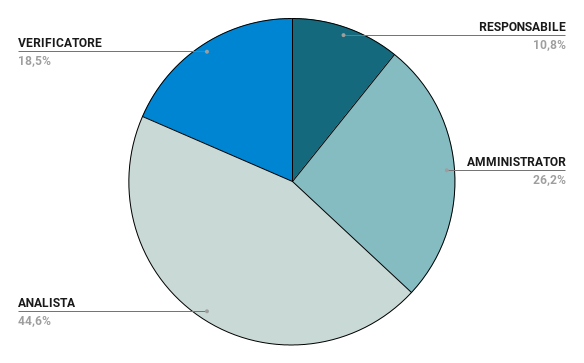
\includegraphics[width=0.8\textwidth]{prev1ruoli.png}
    \caption{Distribuzione dei ruoli primo sprint}
    \label{fig:preventivoorarioprimosprint}
\end{figure}


\newpage

\subsubsection{Preventivo economico}

{
\setlength{\tabcolsep}{10pt}
\renewcommand{\arraystretch}{1.5}
\rowcolors{2}{oddrow}{evenrow}
\begin{table}[h]
    \centering
    \begin{tabularx}{\textwidth}{| l | l | l | X |}
        \hline
        \rowcolor{headerrow} \textbf{\textcolor{white}{Ruolo}} & \textbf{\textcolor{white}{Costo orario}} & \textbf{\textcolor{white}{Ore impiegate}} & \textbf{\textcolor{white}{Costo €}} \\
        \hline
        Responsabile & 30 & 7 & 210\\
        \hline
        Amministratore & 20 & 17  & 340\\
        \hline
        Progettista& 25 & 0  & 0\\
        \hline
        Analista & 25 & 29  & 725\\
        \hline
        Programmatore & 15 & 0  & 0\\
        \hline
        Verificatore & 15 & 12  & 180\\
        \hline
        \cellcolor{headerrow} \textbf{\textcolor{white}{Totale}} &  &  & \textbf{1455}\\
        \hline
        \cellcolor{headerrow} \textbf{\textcolor{white}{Rimanente}} &  &  & \textbf{11530}\\
        \hline
    \end{tabularx}
    \caption{Preventivo economico primo sprint}
    \label{tab:preventivocostiprimosprint}
\end{table}
}

\begin{figure}[h!]
    \centering
    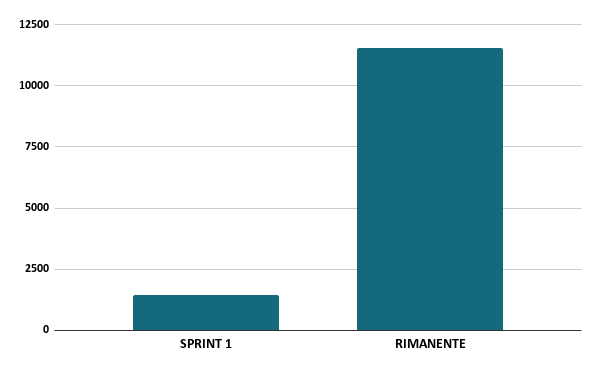
\includegraphics[width=\textwidth]{prev1costo.png}
    \caption{Costo preventivato primo sprint e rimanente}
    \label{fig:preventivocostoprimosprint}
\end{figure}


\newpage


\subsection{Secondo sprint: 2023/11/20 - 2023/12/03}

\subsubsection{Preventivo orario}

{
\setlength{\tabcolsep}{10pt}
\renewcommand{\arraystretch}{1.5}
\rowcolors{2}{oddrow}{evenrow}
\begin{table}[h!]
    \centering
    \begin{tabularx}{\textwidth}{| l | c | c | c | c | c | c | X |}
        \hline
        \rowcolor{headerrow} \textbf{\textcolor{white}{Membro}} & \textbf{\textcolor{white}{R.}} & \textbf{\textcolor{white}{Am.}} & \textbf{\textcolor{white}{Pj.}} & \textbf{\textcolor{white}{An.}} & \textbf{\textcolor{white}{Pg.}} & \textbf{\textcolor{white}{V.}} & \textbf{\textcolor{white}{Totale}} \\
        \hline
        Andrea Cecchin & - & 3 & 3 & - & 3 & - & \textbf{9} \\
        \hline
        Marco Dolzan & - &  & - & 2 & 3 & 4 & \textbf{9} \\
        \hline
        Francesco Ferraioli & - & - & 2 & 5 & - & 2 & \textbf{9} \\
        \hline  
        Francesco Giacomuzzo & 7 & - & - & - & - & 2 & \textbf{9} \\
        \hline
        Leonardo Lago & - & 3 & 3 & - & - & 4 & \textbf{10} \\
        \hline
        Giovanni Menon & - & - & 1 & 5 & 4 & - & \textbf{10} \\
        \hline
        Anna Nordio & - & 2 & - & 5 & 2 & - & \textbf{9} \\
        \hline
    \cellcolor{headerrow} \textbf{\textcolor{white}{Totale}} & \textbf{7} & \textbf{8} & \textbf{9} & \textbf{17} & \textbf{12} & \textbf{12} & \textbf{65} \\
        \hline
    \end{tabularx} 
    \caption{Preventivo orario secondo sprint}
    \label{tab:preventivoorariosecondosprint}
\end{table}
}

\begin{figure}[h!]
    \centering
    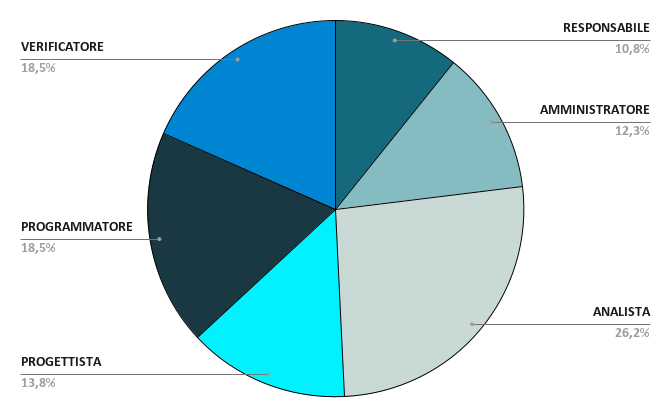
\includegraphics[width=0.8\textwidth]{prev2ruoli.png}
    \caption{Distribuzione dei ruoli secondo sprint}
    \label{fig:preventivoorariosecondosprint}
\end{figure}


\newpage
\subsubsection{Preventivo economico}

{
\setlength{\tabcolsep}{10pt}
\renewcommand{\arraystretch}{1.5}
\rowcolors{2}{oddrow}{evenrow}
\begin{table}[h]
    \centering
    \begin{tabularx}{\textwidth}{| l | l | l | X |}
        \hline
        \rowcolor{headerrow} \textbf{\textcolor{white}{Ruolo}} & \textbf{\textcolor{white}{Costo orario}} & \textbf{\textcolor{white}{Ore impiegate}} & \textbf{\textcolor{white}{Costo €}} \\
        \hline
        Responsabile & 30 & 7 & 210\\
        \hline
        Amministratore & 20 & 8 & 160\\
        \hline
        Progettista& 25 & 9  & 225\\
        \hline
        Analista & 25 & 17  & 425\\
        \hline
        Programmatore & 15 & 12 & 180\\
        \hline
        Verificatore & 15 & 12  & 180\\
        \hline
        \cellcolor{headerrow} \textbf{\textcolor{white}{Totale}} &  &  & \textbf{1380}\\
        \hline
        \cellcolor{headerrow} \textbf{\textcolor{white}{Rimanente}} &  &  & \textbf{10240}\\
        \hline
    \end{tabularx}
    \caption{Preventivo economico secondo sprint}
    \label{tab:preventivocostisecondosprint}
\end{table}
}

\begin{figure}[h!]
    \centering
    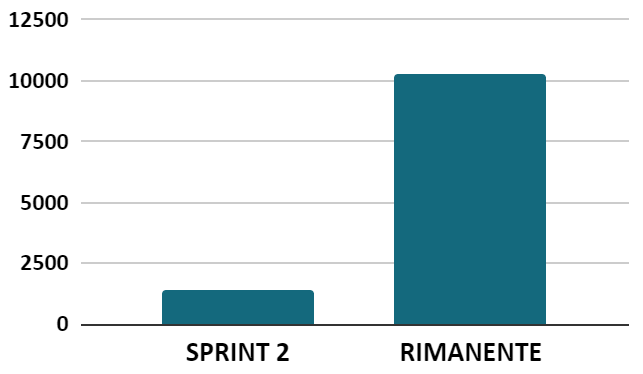
\includegraphics[width=\textwidth]{prev2costo.png}
    \caption{Costo preventivato secondo sprint e rimanente}
    \label{fig:preventivocostosecondosprint}
\end{figure}


\newpage
\subsection{Terzo sprint: 2023/12/04 - 2023/12/17}
\subsubsection{Preventivo orario}
{
\setlength{\tabcolsep}{10pt}
\renewcommand{\arraystretch}{1.5}
\rowcolors{2}{oddrow}{evenrow}
\begin{table}[h!]
    \centering
    \begin{tabularx}{\textwidth}{| l | c | c | c | c | c | c | X |}
        \hline
        \rowcolor{headerrow} \textbf{\textcolor{white}{Membro}} & \textbf{\textcolor{white}{R.}} & \textbf{\textcolor{white}{Am.}} & \textbf{\textcolor{white}{Pj.}} & \textbf{\textcolor{white}{An.}} & \textbf{\textcolor{white}{Pg.}} & \textbf{\textcolor{white}{V.}} & \textbf{\textcolor{white}{Totale}} \\
        \hline
        Andrea Cecchin & - & 1 & - & - & 4 & 4 & \textbf{9} \\
        \hline
        Marco Dolzan & - & 5 & 2 & - & 2 & - & \textbf{9} \\
        \hline
        Francesco Ferraioli & - & - & - & 4 & 3 & 3 & \textbf{10} \\
        \hline  
        Francesco Giacomuzzo & - & - & 2 & 3 & - & 4 & \textbf{9} \\
        \hline
        Leonardo Lago & 7 & - & - & 2 & - & - & \textbf{9} \\
        \hline
        Giovanni Menon & - & 4 & - & 2 & 4 & - & \textbf{10} \\
        \hline
        Anna Nordio & - & - & 2 & 5 & 3 & - & \textbf{10} \\
        \hline
    \cellcolor{headerrow} \textbf{\textcolor{white}{Totale}} & \textbf{7} & \textbf{10} & \textbf{6} & \textbf{16} & \textbf{16} & \textbf{11} & \textbf{66} \\
        \hline
    \end{tabularx} 
    \caption{Preventivo orario terzo sprint}
    \label{tab:preventivoorarioterzosprint}
\end{table}
}

\begin{figure}[h!]
    \centering
    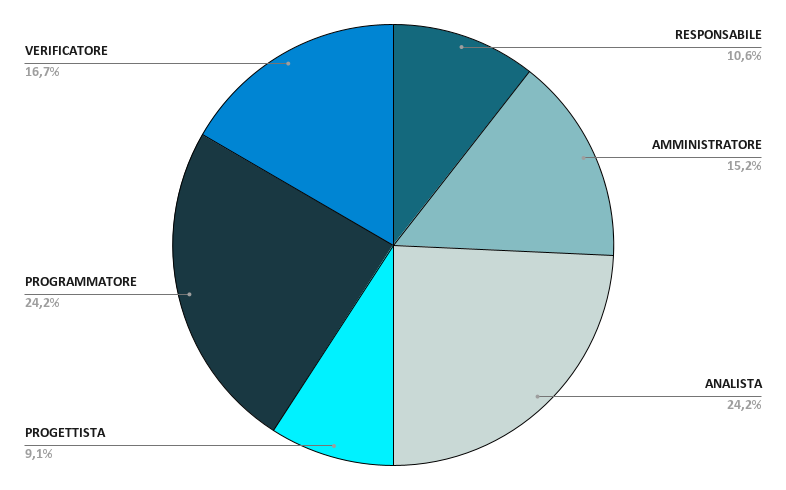
\includegraphics[width=0.9\textwidth]{prev3ruoli.png}
    \caption{Distribuzione dei ruoli terzo sprint}
    \label{fig:preventivoorarioterzosprint}
\end{figure}

\subsubsection{Preventivo economico}
{
\setlength{\tabcolsep}{10pt}
\renewcommand{\arraystretch}{1.5}
\rowcolors{2}{oddrow}{evenrow}
\begin{table}[h]
    \centering
    \begin{tabularx}{\textwidth}{| l | l | l | X |}
        \hline
        \rowcolor{headerrow} \textbf{\textcolor{white}{Ruolo}} & \textbf{\textcolor{white}{Costo orario}} & \textbf{\textcolor{white}{Ore impiegate}} & \textbf{\textcolor{white}{Costo €}} \\
        \hline
        Responsabile & 30 & 7 & 210\\
        \hline
        Amministratore & 20 & 10 & 200\\
        \hline
        Progettista& 25 & 6 & 150\\
        \hline
        Analista & 25 & 16 & 400\\
        \hline
        Programmatore & 15 & 16 & 240\\
        \hline
        Verificatore & 15 & 11 & 165\\
        \hline
        \cellcolor{headerrow} \textbf{\textcolor{white}{Totale}} &  &  & \textbf{1365}\\
        \hline
        \cellcolor{headerrow} \textbf{\textcolor{white}{Rimanente}} &  &  & \textbf{8920}\\
        \hline
    \end{tabularx}
    \caption{Preventivo economico terzo sprint}
    \label{tab:preventivocostiterzosprint}
\end{table}
}

\begin{figure}[h!]
    \centering
    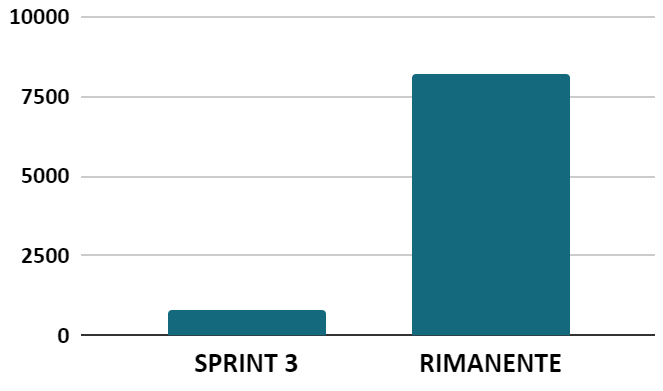
\includegraphics[width=0.9\textwidth]{prev3costo.png}
    \caption{Costo preventivato terzo sprint e rimanente}
    \label{fig:preventivocostoterzosprint}
\end{figure}

\newpage
\subsection{Quarto sprint: 2023/12/18 - 2023/12/31}
\subsubsection{Preventivo orario}
{
\setlength{\tabcolsep}{10pt}
\renewcommand{\arraystretch}{1.5}
\rowcolors{2}{oddrow}{evenrow}
\begin{table}[h!]
    \centering
    \begin{tabularx}{\textwidth}{| l | c | c | c | c | c | c | X |}
        \hline
        \rowcolor{headerrow} \textbf{\textcolor{white}{Membro}} & \textbf{\textcolor{white}{R.}} & \textbf{\textcolor{white}{Am.}} & \textbf{\textcolor{white}{Pj.}} & \textbf{\textcolor{white}{An.}} & \textbf{\textcolor{white}{Pg.}} & \textbf{\textcolor{white}{V.}} & \textbf{\textcolor{white}{Totale}} \\
        \hline
        Andrea Cecchin & - & - & 1 & - & 1 & 4 & \textbf{6} \\
        \hline
        Marco Dolzan & - & - & - & - & 1 & 5 & \textbf{6} \\
        \hline
        Francesco Ferraioli & 5 & 1 & - & - & - & - & \textbf{6} \\
        \hline  
        Francesco Giacomuzzo & - & 3 & - & 2 & 2 & - & \textbf{7} \\
        \hline
        Leonardo Lago & - & - & - & 2 & 4 & - & \textbf{6} \\
        \hline
        Giovanni Menon & - & - & - & 3 & 1 & 2 & \textbf{6} \\
        \hline
        Anna Nordio & - & 1 & - & - & - & 5 & \textbf{6} \\
        \hline
    \cellcolor{headerrow} \textbf{\textcolor{white}{Totale}} & \textbf{5} & \textbf{5} & \textbf{1} & \textbf{7} & \textbf{9} & \textbf{16} & \textbf{43} \\
        \hline
    \end{tabularx} 
    \caption{Preventivo orario quarto sprint}
    \label{tab:preventivoorarioquartosprint}
\end{table}
}

\begin{figure}[h!]
    \centering
    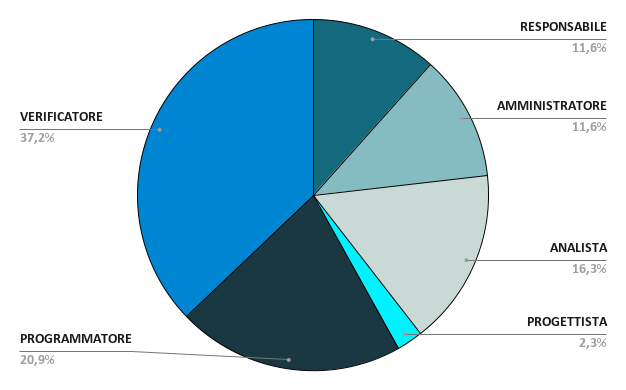
\includegraphics[width=0.9\textwidth]{prev4ruoli.png}
    \caption{Distribuzione dei ruoli quarto sprint}
    \label{fig:preventivoorarioquartosprint}
\end{figure}

\subsubsection{Preventivo economico}
{
\setlength{\tabcolsep}{10pt}
\renewcommand{\arraystretch}{1.5}
\rowcolors{2}{oddrow}{evenrow}
\begin{table}[h]
    \centering
    \begin{tabularx}{\textwidth}{| l | l | l | X |}
        \hline
        \rowcolor{headerrow} \textbf{\textcolor{white}{Ruolo}} & \textbf{\textcolor{white}{Costo orario}} & \textbf{\textcolor{white}{Ore impiegate}} & \textbf{\textcolor{white}{Costo €}} \\
        \hline
        Responsabile & 30 & 5 & 150\\
        \hline
        Amministratore & 20 & 5 & 100\\
        \hline
        Progettista& 25 & 1 & 25\\
        \hline
        Analista & 25 & 7 & 175\\
        \hline
        Programmatore & 15 & 9 & 135\\
        \hline
        Verificatore & 15 & 16 & 240\\
        \hline
        \cellcolor{headerrow} \textbf{\textcolor{white}{Totale}} &  &  & \textbf{825}\\
        \hline
        \cellcolor{headerrow} \textbf{\textcolor{white}{Rimanente}} &  &  & \textbf{8195}\\
        \hline
    \end{tabularx}
    \caption{Preventivo economico quarto sprint}
    \label{tab:preventivocostiquartosprint}
\end{table}
}

\begin{figure}[h!]
    \centering
    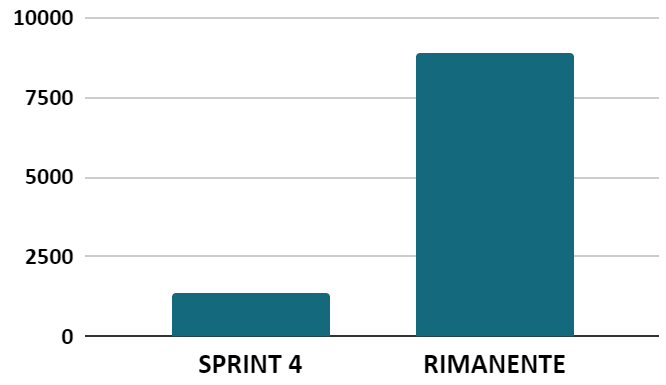
\includegraphics[width=0.9\textwidth]{prev4costo.png}
    \caption{Costo preventivato quarto sprint e rimanente}
    \label{fig:preventivocostoquartosprint}
\end{figure}

\newpage

\subsection{Quinto sprint: 2024/01/01 - 2024/01/14}
\subsubsection{Preventivo orario}
{
\setlength{\tabcolsep}{10pt}
\renewcommand{\arraystretch}{1.5}
\rowcolors{2}{oddrow}{evenrow}
\begin{table}[h!]
    \centering
    \begin{tabularx}{\textwidth}{| l | c | c | c | c | c | c | X |}
        \hline
        \rowcolor{headerrow} \textbf{\textcolor{white}{Membro}} & \textbf{\textcolor{white}{R.}} & \textbf{\textcolor{white}{Am.}} & \textbf{\textcolor{white}{Pj.}} & \textbf{\textcolor{white}{An.}} & \textbf{\textcolor{white}{Pg.}} & \textbf{\textcolor{white}{V.}} & \textbf{\textcolor{white}{Totale}} \\
        \hline
        Andrea Cecchin & 5 & - & - & - & - & - & \textbf{5} \\
        \hline
        Marco Dolzan & - & - & - & 3 & - & 2 & \textbf{5} \\
        \hline
        Francesco Ferraioli & - & 1 & - & - & 2 & 2 & \textbf{5} \\
        \hline  
        Francesco Giacomuzzo & - & 2 & - & - & 3 & - & \textbf{5} \\
        \hline
        Leonardo Lago & - & - & 2 & - & - & 3 & \textbf{5} \\
        \hline
        Giovanni Menon & - & - & 2 & 2 & - & 3 & \textbf{7} \\
        \hline
        Anna Nordio & - & 2 & - & - & - & 4 & \textbf{6} \\
        \hline
    \cellcolor{headerrow} \textbf{\textcolor{white}{Totale}} & \textbf{5} & \textbf{5} & \textbf{4} & \textbf{5} & \textbf{5} & \textbf{14} & \textbf{38} \\
        \hline
    \end{tabularx} 
    \caption{Preventivo orario quinto sprint}
    \label{tab:preventivoorarioquintosprint}
\end{table}
}

\begin{figure}[h!]
    \centering
    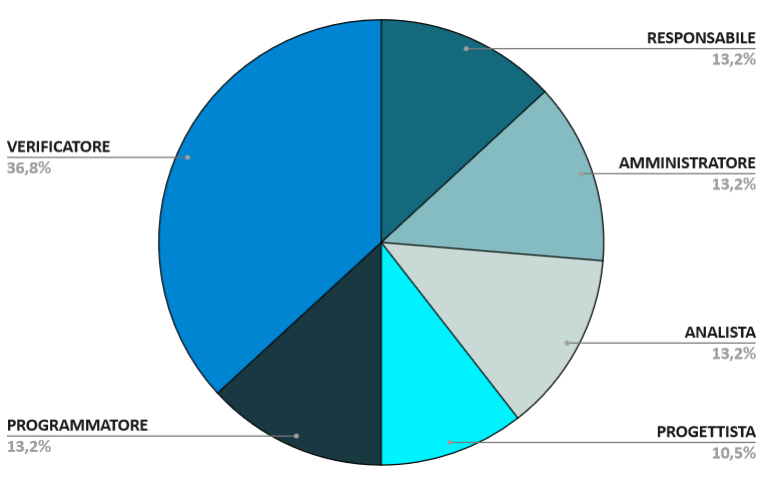
\includegraphics[width=0.9\textwidth]{prev5ruoli.png}
    \caption{Distribuzione dei ruoli quinto sprint}
    \label{fig:preventivoorarioquintosprint}
\end{figure}

\subsubsection{Preventivo economico}
{
\setlength{\tabcolsep}{10pt}
\renewcommand{\arraystretch}{1.5}
\rowcolors{2}{oddrow}{evenrow}
\begin{table}[h]
    \centering
    \begin{tabularx}{\textwidth}{| l | l | l | X |}
        \hline
        \rowcolor{headerrow} \textbf{\textcolor{white}{Ruolo}} & \textbf{\textcolor{white}{Costo orario}} & \textbf{\textcolor{white}{Ore impiegate}} & \textbf{\textcolor{white}{Costo €}} \\
        \hline
        Responsabile & 30 & 5 & 150\\
        \hline
        Amministratore & 20 & 5 & 100\\
        \hline
        Progettista& 25 & 4 & 100\\
        \hline
        Analista & 25 & 5 & 125\\
        \hline
        Programmatore & 15 & 5 & 75\\
        \hline
        Verificatore & 15 & 14 & 210\\
        \hline
        \cellcolor{headerrow} \textbf{\textcolor{white}{Totale}} &  &  & \textbf{760}\\
        \hline
        \cellcolor{headerrow} \textbf{\textcolor{white}{Rimanente}} &  &  & \textbf{7505}\\
        \hline
    \end{tabularx}
    \caption{Preventivo economico quinto sprint}
    \label{tab:preventivocostiquintosprint}
\end{table}
}

\begin{figure}[h!]
    \centering
    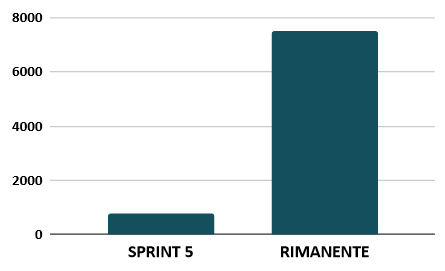
\includegraphics[width=0.9\textwidth]{prev5costo.png}
    \caption{Costo preventivato quinto sprint e rimanente}
    \label{fig:preventivocostoquintosprint}
\end{figure}

\newpage

\subsection{Sesto sprint: 2024/01/15 - 2024/01/28}
\subsubsection{Preventivo orario}
{
\setlength{\tabcolsep}{10pt}
\renewcommand{\arraystretch}{1.5}
\rowcolors{2}{oddrow}{evenrow}
\begin{table}[h!]
    \centering
    \begin{tabularx}{\textwidth}{| l | c | c | c | c | c | c | X |}
        \hline
        \rowcolor{headerrow} \textbf{\textcolor{white}{Membro}} & \textbf{\textcolor{white}{R.}} & \textbf{\textcolor{white}{Am.}} & \textbf{\textcolor{white}{Pj.}} & \textbf{\textcolor{white}{An.}} & \textbf{\textcolor{white}{Pg.}} & \textbf{\textcolor{white}{V.}} & \textbf{\textcolor{white}{Totale}} \\
        \hline
        Andrea Cecchin & - & - & 2 & 2 & - & 2 & \textbf{6} \\
        \hline
        Marco Dolzan & 4 & - & - & - & - & - & \textbf{4} \\
        \hline
        Francesco Ferraioli & - & - & 2 & - & 2 & 2 & \textbf{6} \\
        \hline  
        Francesco Giacomuzzo & - & - & - & 2 & 3 & - & \textbf{5} \\
        \hline
        Leonardo Lago & - & - & 1 & - & 2 & 2 & \textbf{5} \\
        \hline
        Giovanni Menon & - & - & 3 & - & 2 & 1 & \textbf{6} \\
        \hline
        Anna Nordio & - & - & 4 & - & 1 & 3 & \textbf{8} \\
        \hline
    \cellcolor{headerrow} \textbf{\textcolor{white}{Totale}} & \textbf{4} & \textbf{0} & \textbf{12} & \textbf{4} & \textbf{10} & \textbf{10} & \textbf{40} \\
        \hline
    \end{tabularx} 
    \caption{Preventivo orario sesto sprint}
    \label{tab:preventivoorariosestosprint}
\end{table}
}

\begin{figure}[h!]
    \centering
    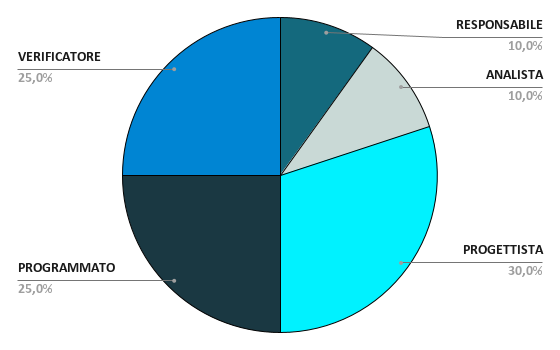
\includegraphics[width=0.9\textwidth]{prev6ruoli.png}
    \caption{Distribuzione dei ruoli sesto sprint}
    \label{fig:preventivoorariosestosprint}
\end{figure}

\subsubsection{Preventivo economico}
{
\setlength{\tabcolsep}{10pt}
\renewcommand{\arraystretch}{1.5}
\rowcolors{2}{oddrow}{evenrow}
\begin{table}[h]
    \centering
    \begin{tabularx}{\textwidth}{| l | l | l | X |}
        \hline
        \rowcolor{headerrow} \textbf{\textcolor{white}{Ruolo}} & \textbf{\textcolor{white}{Costo orario}} & \textbf{\textcolor{white}{Ore impiegate}} & \textbf{\textcolor{white}{Costo €}} \\
        \hline
        Responsabile & 30 & 4 & 120\\
        \hline
        Amministratore & 20 & 0 & 0\\
        \hline
        Progettista& 25 & 12 & 300\\
        \hline
        Analista & 25 & 4 & 100\\
        \hline
        Programmatore & 15 & 10 & 150\\
        \hline
        Verificatore & 15 & 10 & 150\\
        \hline
        \cellcolor{headerrow} \textbf{\textcolor{white}{Totale}} &  &  & \textbf{820}\\
        \hline
        \cellcolor{headerrow} \textbf{\textcolor{white}{Rimanente}} &  &  & \textbf{6645}\\
        \hline
    \end{tabularx}
    \caption{Preventivo economico sesto sprint}
    \label{tab:preventivocostisestosprint}
\end{table}
}

\begin{figure}[h!]
    \centering
    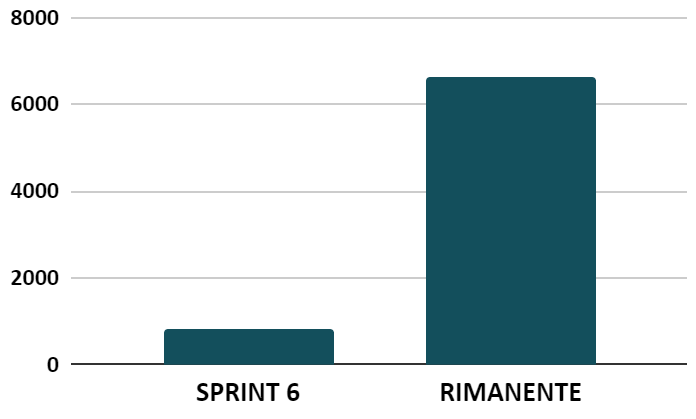
\includegraphics[width=0.9\textwidth]{prev6costo.png}
    \caption{Costo preventivato sesto sprint e rimanente}
    \label{fig:preventivocostosestosprint}
\end{figure}


\newpage

\subsection{Settimo sprint: 2024/01/29 - 2024/02/11}
\subsubsection{Preventivo orario}
{
\setlength{\tabcolsep}{10pt}
\renewcommand{\arraystretch}{1.5}
\rowcolors{2}{oddrow}{evenrow}
\begin{table}[h!]
    \centering
    \begin{tabularx}{\textwidth}{| l | c | c | c | c | c | c | X |}
        \hline
        \rowcolor{headerrow} \textbf{\textcolor{white}{Membro}} & \textbf{\textcolor{white}{R.}} & \textbf{\textcolor{white}{Am.}} & \textbf{\textcolor{white}{Pj.}} & \textbf{\textcolor{white}{An.}} & \textbf{\textcolor{white}{Pg.}} & \textbf{\textcolor{white}{V.}} & \textbf{\textcolor{white}{Totale}} \\
        \hline
        Andrea Cecchin & - & - & 3 & - & - & 3 & \textbf{6} \\
        \hline
        Marco Dolzan & - & - & 3 & - & - & 3 & \textbf{6} \\
        \hline
        Francesco Ferraioli & - & - & 4 & - & - & 2 & \textbf{6} \\
        \hline  
        Francesco Giacomuzzo & - & - & 4 & 2 & - & - & \textbf{6} \\
        \hline
        Leonardo Lago & - & - & 2 & - & - & 3 & \textbf{5} \\
        \hline
        Giovanni Menon & - & 2 & - & - & - & 3 & \textbf{5} \\
        \hline
        Anna Nordio & 5 & - & - & 1 & - & - & \textbf{6} \\
        \hline
    \cellcolor{headerrow} \textbf{\textcolor{white}{Totale}} & \textbf{5} & \textbf{2} & \textbf{16} & \textbf{3} & \textbf{0} & \textbf{14} & \textbf{40} \\
        \hline
    \end{tabularx} 
    \caption{Preventivo orario settimo sprint}
    \label{tab:preventivoorariosettimosprint}
\end{table}
}

\begin{figure}[h!]
    \centering
    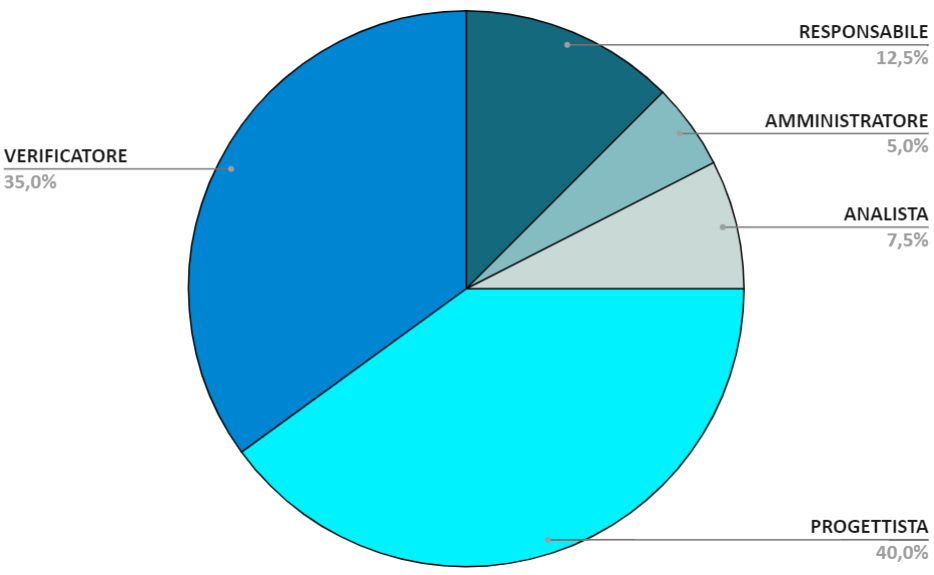
\includegraphics[width=0.9\textwidth]{prev7ruoli.png}
    \caption{Distribuzione dei ruoli settimo sprint}
    \label{fig:preventivoorariosettimosprint}
\end{figure}

\subsubsection{Preventivo economico}
{
\setlength{\tabcolsep}{10pt}
\renewcommand{\arraystretch}{1.5}
\rowcolors{2}{oddrow}{evenrow}
\begin{table}[h]
    \centering
    \begin{tabularx}{\textwidth}{| l | l | l | X |}
        \hline
        \rowcolor{headerrow} \textbf{\textcolor{white}{Ruolo}} & \textbf{\textcolor{white}{Costo orario}} & \textbf{\textcolor{white}{Ore impiegate}} & \textbf{\textcolor{white}{Costo €}} \\
        \hline
        Responsabile & 30 & 5 & 150\\
        \hline
        Amministratore & 20 & 2 & 40\\
        \hline
        Progettista& 25 & 16 & 400\\
        \hline
        Analista & 25 & 3 & 75\\
        \hline
        Programmatore & 15 & 0 & 0\\
        \hline
        Verificatore & 15 & 14 & 210\\
        \hline
        \cellcolor{headerrow} \textbf{\textcolor{white}{Totale}} &  &  & \textbf{875}\\
        \hline
        \cellcolor{headerrow} \textbf{\textcolor{white}{Rimanente}} &  &  & \textbf{5805}\\
        \hline
    \end{tabularx}
    \caption{Preventivo economico settimo sprint}
    \label{tab:preventivocostisettimosprint}
\end{table}
}

\begin{figure}[h!]
    \centering
    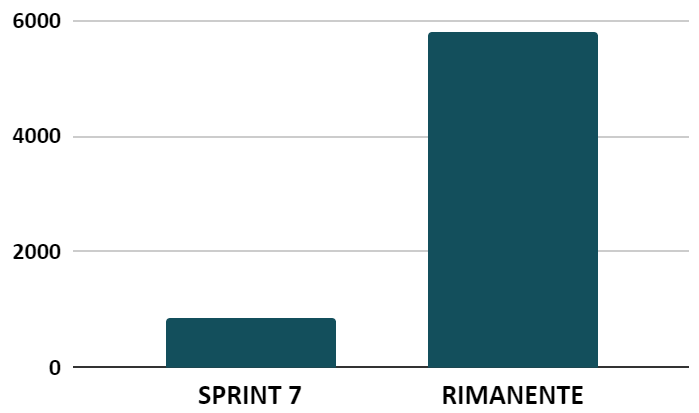
\includegraphics[width=0.9\textwidth]{prev7costo.png}
    \caption{Costo preventivato settimo sprint e rimanente}
    \label{fig:preventivocostosettimosprint}
\end{figure}


\newpage
\subsection{Preventivo a finire} \label{sec:risuddivisione}
\setlength{\tabcolsep}{10pt}
\renewcommand{\arraystretch}{1.5}
\rowcolors{2}{oddrow}{evenrow}
\begin{table}[h!]
    \centering
    \begin{tabularx}{\textwidth}{| X | c | c |}
        \hline
        \rowcolor{headerrow} \textbf{\textcolor{white}{Membro}} & \textbf{\textcolor{white}{Ore effettuate}} & \textbf{\textcolor{white}{Ore rimanenti}} \\
        \hline
        Andrea Cecchin & 49 & 44 \\
        \hline
        Marco Dolzan & 46 & 47 \\
        \hline
        Francesco Ferraioli & 51 & 42 \\
        \hline  
        Francesco Giacomuzzo & 46 & 47 \\
        \hline
        Leonardo Lago & 49 & 44\\
        \hline
        Giovanni Menon & 53 & 40\\
        \hline
        Anna Nordio & 51 & 42\\
        \hline
    \end{tabularx} 
    \caption{Ore di lavoro effettuate al termine della revisione RTB}
    \label{tab:orefatte}
\end{table}
\begin{figure}[h!]
    \centering
    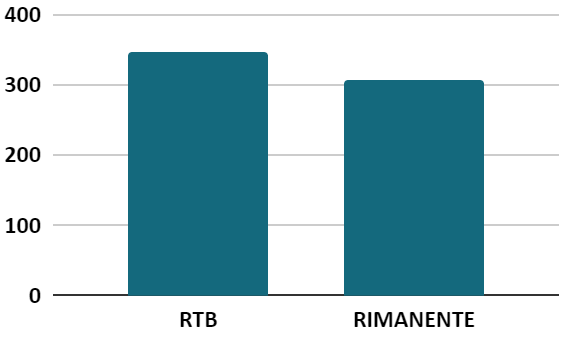
\includegraphics[width=0.6\textwidth]{oreTotaliRTB.png}
    \caption{Ore effettuate al termine dell'RTB e rimanenti}
    \label{fig:oreeffettiveRTB}
\end{figure}
\noindent Nel preventivo iniziale il ruolo del responsabile era stato sottostimato, assegnando quindi un numero non adeguato di ore produttive. Allo stesso modo, le ore destinate alla verifica al termine della revisione RTB non risultavano essere abbastanza. Al contrario, per quanto riguarda le ore di analisi, c'era stata un evidente sovrastima all'inizio del progetto. Per questo motivo è stato deciso di risuddividere le ore in modo da restare dentro il budget di \textit{12.985€} e in modo che ogni \ccgloss{componente} del gruppo raggiunga e non superi le 93 ore produttive.\\
Al termine della revisone RTB la suddivisione delle ore rimanenti per ogni ruolo era la seguente:
\setlength{\tabcolsep}{10pt}
\renewcommand{\arraystretch}{1.4}
\rowcolors{2}{oddrow}{evenrow}
\begin{table}[h!]
    \centering
    \begin{tabularx}{\textwidth}{| l | c | c | c | c | c | c | X |}
        \hline
        \rowcolor{headerrow} \textbf{\textcolor{white}{Membro}} & \textbf{\textcolor{white}{R.}} & \textbf{\textcolor{white}{Am.}} & \textbf{\textcolor{white}{Pj.}} & \textbf{\textcolor{white}{An.}} & \textbf{\textcolor{white}{Pg.}} & \textbf{\textcolor{white}{V.}}&\textbf{\textcolor{white}{Totale}} \\
        \hline
        Andrea Cecchin & 3 & 1 & 12 & 3 & 13 & 11 & \textbf{44}\\
        \hline
        Marco Dolzan & 3 & 3 & 13 & 3 & 15 & 10 & \textbf{47}\\
        \hline
        Francesco Ferraioli & 5 & - & 8& 3 & 16 & 10& \textbf{42}\\
        \hline  
        Francesco Giacomuzzo & 1 & 2 & 12 & 2 & 17 & 13 & \textbf{47}\\
        \hline
        Leonardo Lago & 2 & 2 & 10 & 2 & 17 & 11& \textbf{44}\\
        \hline
        Giovanni Menon & - & 1 & 12 & 2 & 13 & 12& \textbf{40}\\
        \hline
        Anna Nordio & 4 & - & 15 & 2 & 13 & 8& \textbf{42}\\
        \hline
    \cellcolor{headerrow} \textbf{\textcolor{white}{Totale}} & \textbf{18} & \textbf{9} & \textbf{79} & \textbf{17} & \textbf{105} & \textbf{74}& \textbf{302}\\
        \hline
    \end{tabularx} 
    \caption{Suddivisione oraria dei ruoli per componente al termine della revisione RTB}
    \label{tab:ruoliprerisuddivisione}
\end{table}\\

\setlength{\tabcolsep}{10pt}
\renewcommand{\arraystretch}{1.4}
\rowcolors{2}{oddrow}{evenrow}
\noindent A seguito della nuova suddivisione delle ore per ogni ruolo:
\begin{table}[h!]
    \centering
    \begin{tabularx}{\textwidth}{| l | c | c | c | c | c | c | X |}
        \hline
        \rowcolor{headerrow} \textbf{\textcolor{white}{Membro}} & \textbf{\textcolor{white}{R.}} & \textbf{\textcolor{white}{Am.}} & \textbf{\textcolor{white}{Pj.}} & \textbf{\textcolor{white}{An.}} & \textbf{\textcolor{white}{Pg.}} & \textbf{\textcolor{white}{V.}}&\textbf{\textcolor{white}{Totale}} \\
        \hline
        Andrea Cecchin & 4 & 1 & 12 & 2 & 14 & 11 & \textbf{44}\\
        \hline
        Marco Dolzan & 4 & 3 & 13 & 2 & 14 & 11 & \textbf{47}\\
        \hline
        Francesco Ferraioli & 4 & - & 8 & 2 & 15 & 13 &  \textbf{42}\\
        \hline  
        Francesco Giacomuzzo & 4 & 2 & 12 & - & 16 & 13 & \textbf{47}\\
        \hline
        Leonardo Lago & 4 & 2 & 10 & - & 16 & 12 &  \textbf{44}\\
        \hline
        Giovanni Menon & - & 1 & 12 & 2 & 13 & 12 &  \textbf{40}\\
        \hline
        Anna Nordio & 4 & - & 13 & 2 & 12 & 11 &  \textbf{42}\\
        \hline
    \cellcolor{headerrow} \textbf{\textcolor{white}{Totale}} & \textbf{24} & \textbf{9} & \textbf{77} & \textbf{10} & \textbf{100} & \textbf{82} & \textbf{302}\\
        \hline
    \end{tabularx} 
    \caption{Risuddivisione oraria dei ruoli per componente}
    \label{tab:risuddivisione}
\end{table}
\newpage

\section{Product Baseline}

\subsection{Ottavo sprint: 2024/02/12 - 2024/02/25}
\subsubsection{Preventivo orario}

{
\setlength{\tabcolsep}{10pt}
\renewcommand{\arraystretch}{1.5}
\rowcolors{2}{oddrow}{evenrow}
\begin{table}[h!]
    \centering
    \begin{tabularx}{\textwidth}{| l | c | c | c | c | c | c | X |}
        \hline
        \rowcolor{headerrow} \textbf{\textcolor{white}{Membro}} & \textbf{\textcolor{white}{R.}} & \textbf{\textcolor{white}{Am.}} & \textbf{\textcolor{white}{Pj.}} & \textbf{\textcolor{white}{An.}} & \textbf{\textcolor{white}{Pg.}} & \textbf{\textcolor{white}{V.}} & \textbf{\textcolor{white}{Totale}} \\
        \hline
        %             respo-amm-pj-analis-progr-verifi
        Andrea Cecchin & - & - & 6 & 1 & - & 2 & \textbf{9} \\
        \hline
        Marco Dolzan & - & 1 & 1 & - & - & 3 & \textbf{5} \\
        \hline
        Francesco Ferraioli & - & - & 5 & 2 & 2 & - & \textbf{9} \\
        \hline  
        Francesco Giacomuzzo & 4 & 1 & - & - & - & - & \textbf{5} \\
        \hline
        Leonardo Lago & - & 2 & 4 & - & 3 & - & \textbf{9} \\
        \hline
        Giovanni Menon & - & 1 & 5 & - & 3 & - & \textbf{9} \\
        \hline
        Anna Nordio & - & - & 2 & - & 3 & 4 & \textbf{9} \\
        \hline
    \cellcolor{headerrow} \textbf{\textcolor{white}{Totale}} & \textbf{4} & \textbf{5} & \textbf{23} & \textbf{3} & \textbf{11} & \textbf{9} & \textbf{55} \\
        \hline
    \end{tabularx} 
    \caption{Preventivo orario ottavo sprint}
    \label{tab:preventivoorarioottavosprint}
\end{table}
}

\begin{figure}[h!]
    \centering
    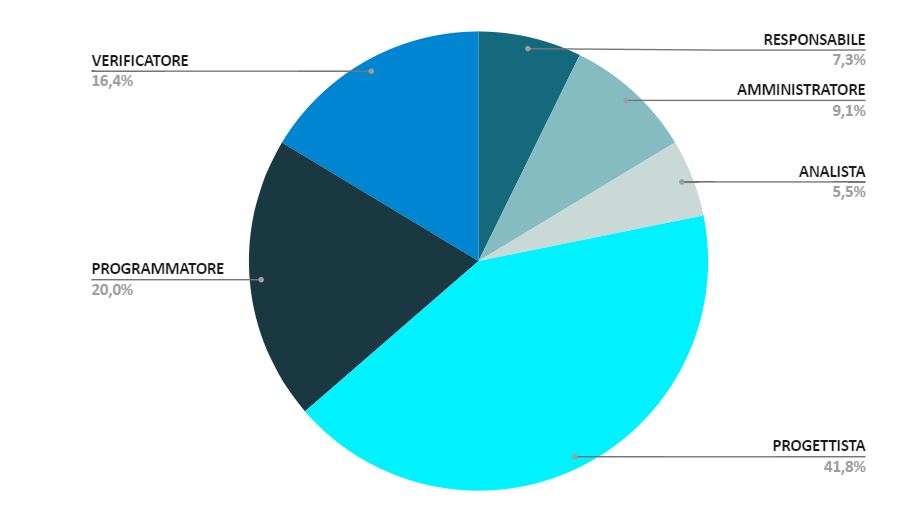
\includegraphics[width=0.8\textwidth]{prev8ruoli.png}
    \caption{Distribuzione dei ruoli ottavo sprint}
    \label{fig:preventivoorarioottavosprint}
\end{figure}


\newpage

\subsubsection{Preventivo economico}

{
\setlength{\tabcolsep}{10pt}
\renewcommand{\arraystretch}{1.5}
\rowcolors{2}{oddrow}{evenrow}
\begin{table}[h]
    \centering
    \begin{tabularx}{\textwidth}{| l | l | l | X |}
        \hline
        \rowcolor{headerrow} \textbf{\textcolor{white}{Ruolo}} & \textbf{\textcolor{white}{Costo orario}} & \textbf{\textcolor{white}{Ore impiegate}} & \textbf{\textcolor{white}{Costo €}} \\
        \hline
        Responsabile & 30 & 4 & 120\\
        \hline
        Amministratore & 20 & 5 & 100\\
        \hline
        Progettista& 25 & 23  & 575\\
        \hline
        Analista & 25 & 3& 75\\
        \hline
        Programmatore & 15 & 11 & 165\\
        \hline
        Verificatore & 15 & 9 & 135\\
        \hline
        \cellcolor{headerrow} \textbf{\textcolor{white}{Totale}} &  &  & \textbf{1170}\\
        \hline
        \cellcolor{headerrow} \textbf{\textcolor{white}{Rimanente}} &  &  & \textbf{4635}\\
        \hline
    \end{tabularx}
    \caption{Preventivo economico ottavo sprint}
    \label{tab:preventivocostiottavosprint}
\end{table}
}

\begin{figure}[h!]
    \centering
    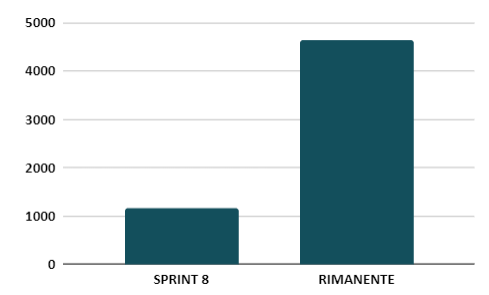
\includegraphics[width=\textwidth]{prev8costo.png}
    \caption{Costo preventivato ottavo sprint e rimanente}
    \label{fig:preventivocostoottavosprint}
\end{figure}


\subsection{Nono sprint: 2024/02/26 - 2024/03/10}
\subsubsection{Preventivo orario}

{
\setlength{\tabcolsep}{10pt}
\renewcommand{\arraystretch}{1.5}
\rowcolors{2}{oddrow}{evenrow}
\begin{table}[h!]
    \centering
    \begin{tabularx}{\textwidth}{| l | c | c | c | c | c | c | X |}
        \hline
        \rowcolor{headerrow} \textbf{\textcolor{white}{Membro}} & \textbf{\textcolor{white}{R.}} & \textbf{\textcolor{white}{Am.}} & \textbf{\textcolor{white}{Pj.}} & \textbf{\textcolor{white}{An.}} & \textbf{\textcolor{white}{Pg.}} & \textbf{\textcolor{white}{V.}} & \textbf{\textcolor{white}{Totale}} \\
        \hline
        %             respo-amm-pj-analis-progr-verifi
        Andrea Cecchin & - & - & 4 & - & 5 & 3 & \textbf{12} \\
        \hline
        Marco Dolzan & - & - & 6 & - & 6 & - & \textbf{12} \\
        \hline
        Francesco Ferraioli & - & - & 2 & - & 7 & 3 & \textbf{12} \\
        \hline  
        Francesco Giacomuzzo & - & - & 4 & - & 5 & 3 & \textbf{12} \\
        \hline
        Leonardo Lago & 4 & - & 4 & - & 4 & - & \textbf{12} \\
        \hline
        Giovanni Menon & - & - & 4 & - & 5 & 3 & \textbf{12} \\
        \hline
        Anna Nordio & - & - & 5 & - & 5 & - & \textbf{10} \\
        \hline
    \cellcolor{headerrow} \textbf{\textcolor{white}{Totale}} & \textbf{4} & \textbf{0} & \textbf{29} & \textbf{0} & \textbf{37} & \textbf{12} & \textbf{82} \\
        \hline
    \end{tabularx} 
    \caption{Preventivo orario nono sprint}
    \label{tab:preventivoorariononosprint}
\end{table}
}

\begin{figure}[h!]
    \centering
    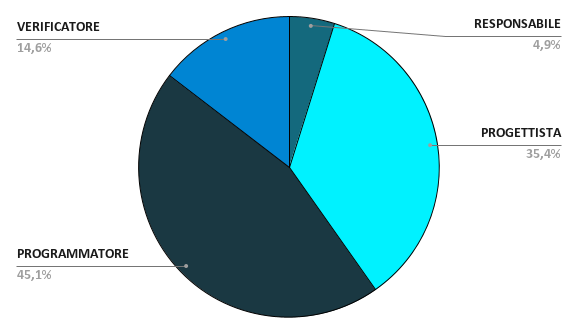
\includegraphics[width=0.8\textwidth]{prev9ruoli.png}
    \caption{Distribuzione dei ruoli nono sprint}
    \label{fig:preventivoorariononosprint}
\end{figure}


\newpage

\subsubsection{Preventivo economico}

{
\setlength{\tabcolsep}{10pt}
\renewcommand{\arraystretch}{1.5}
\rowcolors{2}{oddrow}{evenrow}
\begin{table}[h]
    \centering
    \begin{tabularx}{\textwidth}{| l | l | l | X |}
        \hline
        \rowcolor{headerrow} \textbf{\textcolor{white}{Ruolo}} & \textbf{\textcolor{white}{Costo orario}} & \textbf{\textcolor{white}{Ore impiegate}} & \textbf{\textcolor{white}{Costo €}} \\
        \hline
        Responsabile & 30 & 4 & 120\\
        \hline
        Amministratore & 20 & 0 & 0\\
        \hline
        Progettista& 25 & 29 & 725\\
        \hline
        Analista & 25 & 0 & 0\\
        \hline
        Programmatore & 15 & 37 & 555\\
        \hline
        Verificatore & 15 & 12 & 180\\
        \hline
        \cellcolor{headerrow} \textbf{\textcolor{white}{Totale}} &  &  & \textbf{1580}\\
        \hline
        \cellcolor{headerrow} \textbf{\textcolor{white}{Rimanente}} &  &  & \textbf{3395}\\
        \hline
    \end{tabularx}
    \caption{Preventivo economico nono sprint}
    \label{tab:preventivocostinonosprint}
\end{table}
}

\begin{figure}[h!]
    \centering
    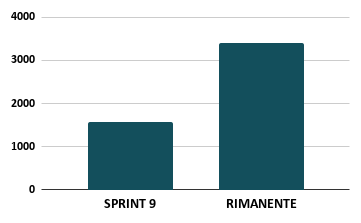
\includegraphics[width=\textwidth]{prev9costo.png}
    \caption{Costo preventivato nono sprint e rimanente}
    \label{fig:preventivocostononosprint}
\end{figure}

\subsection{Decimo sprint: 2024/03/11 - 2024/03/24}
\subsubsection{Preventivo orario}

{
\setlength{\tabcolsep}{10pt}
\renewcommand{\arraystretch}{1.5}
\rowcolors{2}{oddrow}{evenrow}
\begin{table}[h!]
    \centering
    \begin{tabularx}{\textwidth}{| l | c | c | c | c | c | c | X |}
        \hline
        \rowcolor{headerrow} \textbf{\textcolor{white}{Membro}} & \textbf{\textcolor{white}{R.}} & \textbf{\textcolor{white}{Am.}} & \textbf{\textcolor{white}{Pj.}} & \textbf{\textcolor{white}{An.}} & \textbf{\textcolor{white}{Pg.}} & \textbf{\textcolor{white}{V.}} & \textbf{\textcolor{white}{Totale}} \\
        \hline
        %             respo-amm-pj-analis-progr-verifi
        Andrea Cecchin & - & 1 & 3 & 1 & 4 & 2 & \textbf{11} \\
        \hline
        Marco Dolzan & - & - & 4 & - & 6 & 2 & \textbf{12} \\
        \hline
        Francesco Ferraioli & 4 & - & 2 & - & 4 & - & \textbf{10} \\
        \hline  
        Francesco Giacomuzzo & - & - & 4 & - & 4 & 2 & \textbf{10} \\
        \hline
        Leonardo Lago & - & - & 1 & - & 5 & 5 & \textbf{11} \\
        \hline
        Giovanni Menon & - & - & 3 & - & 5 & 3 & \textbf{11} \\
        \hline
        Anna Nordio & - & - & 5 & - & 5 & - & \textbf{10} \\
        \hline
    \cellcolor{headerrow} \textbf{\textcolor{white}{Totale}} & \textbf{4} & \textbf{1} & \textbf{22} & \textbf{1} & \textbf{33} & \textbf{14} & \textbf{75} \\
        \hline
    \end{tabularx} 
    \caption{Preventivo orario decimo sprint}
    \label{tab:preventivoorariodecimosprint}
\end{table}
}

\begin{figure}[h!]
    \centering
    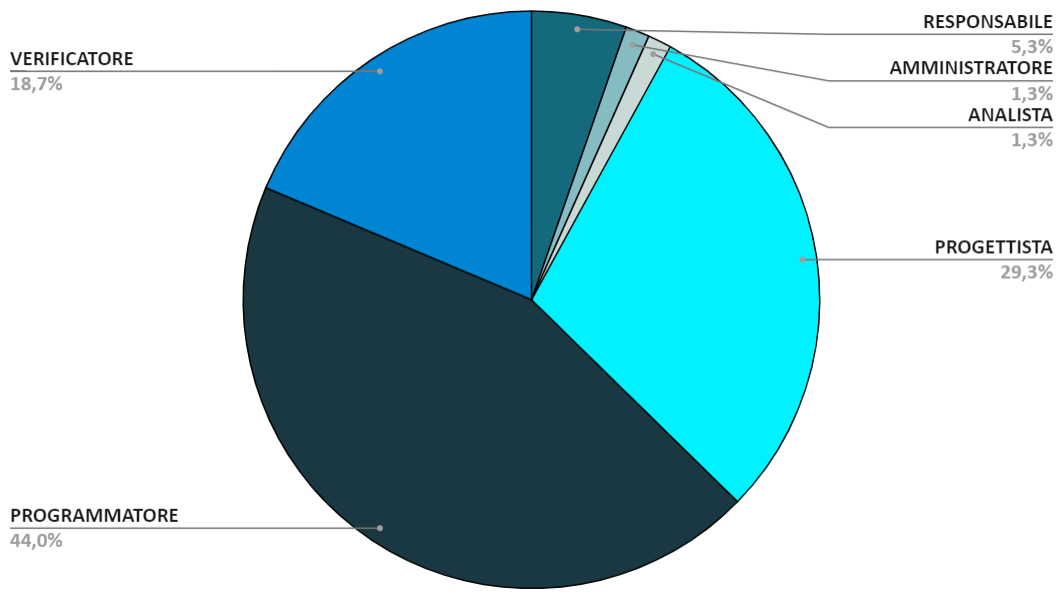
\includegraphics[width=0.9\textwidth]{prev10ruoli.png}
    \caption{Distribuzione dei ruoli decimo sprint}
    \label{fig:preventivoorariodecimosprint}
\end{figure}


\newpage

\subsubsection{Preventivo economico}

{
\setlength{\tabcolsep}{10pt}
\renewcommand{\arraystretch}{1.5}
\rowcolors{2}{oddrow}{evenrow}
\begin{table}[h]
    \centering
    \begin{tabularx}{\textwidth}{| l | l | l | X |}
        \hline
        \rowcolor{headerrow} \textbf{\textcolor{white}{Ruolo}} & \textbf{\textcolor{white}{Costo orario}} & \textbf{\textcolor{white}{Ore impiegate}} & \textbf{\textcolor{white}{Costo €}} \\
        \hline
        Responsabile & 30 & 4 & 120\\
        \hline
        Amministratore & 20 & 1 & 20\\
        \hline
        Progettista& 25 & 22 & 550\\
        \hline
        Analista & 25 & 1 & 25\\
        \hline
        Programmatore & 15 & 33 & 495\\
        \hline
        Verificatore & 15 & 14 & 210\\
        \hline
        \cellcolor{headerrow} \textbf{\textcolor{white}{Totale}} &  &  & \textbf{1420}\\
        \hline
        \cellcolor{headerrow} \textbf{\textcolor{white}{Rimanente}} &  &  & \textbf{2090}\\
        \hline
    \end{tabularx}
    \caption{Preventivo economico decimo sprint}
    \label{tab:preventivocostidecimosprint}
\end{table}
}

\begin{figure}[h!]
    \centering
    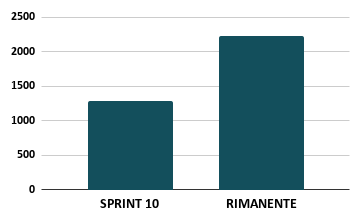
\includegraphics[width=\textwidth]{prev10costo.png}
    \caption{Costo preventivato decimo sprint e rimanente}
    \label{fig:preventivocostodecimosprint}
\end{figure}

\newpage

\subsection{Undicesimo sprint: 2024/03/25 - 2024/04/14}
\subsubsection{Preventivo orario}

{
\setlength{\tabcolsep}{10pt}
\renewcommand{\arraystretch}{1.5}
\rowcolors{2}{oddrow}{evenrow}
\begin{table}[h!]
    \centering
    \begin{tabularx}{\textwidth}{| l | c | c | c | c | c | c | X |}
        \hline
        \rowcolor{headerrow} \textbf{\textcolor{white}{Membro}} & \textbf{\textcolor{white}{R.}} & \textbf{\textcolor{white}{Am.}} & \textbf{\textcolor{white}{Pj.}} & \textbf{\textcolor{white}{An.}} & \textbf{\textcolor{white}{Pg.}} & \textbf{\textcolor{white}{V.}} & \textbf{\textcolor{white}{Totale}} \\
        \hline
        %             respo-amm-pj-analis-progr-verifi
        Andrea Cecchin & 5 & - & - & - & - & 3 & \textbf{8} \\
        \hline
        Marco Dolzan & - & 2 & - & - & 5 & 5 & \textbf{12}  \\
        \hline
        Francesco Ferraioli & - & - & - & - & 3 & 5 & \textbf{8} \\
        \hline  
        Francesco Giacomuzzo & - & 1 & - & - & 5 & 4 & \textbf{10}  \\
        \hline
        Leonardo Lago & - & - & - & - & 5 & 5 & \textbf{10} \\
        \hline
        Giovanni Menon & - & - & 1 & - & 4 & 3 & \textbf{8}  \\
        \hline
        Anna Nordio & - & - & - & - & 4 & 6 & \textbf{10}  \\
        \hline
    \cellcolor{headerrow} \textbf{\textcolor{white}{Totale}} & \textbf{5} & \textbf{3} & \textbf{1} & \textbf{0} & \textbf{26} & \textbf{31} & \textbf{66} \\
        \hline
    \end{tabularx} 
    \caption{Preventivo orario undicesimo sprint}
    \label{tab:preventivoorario11sprint}
\end{table}
}

\begin{figure}[h!]
    \centering
    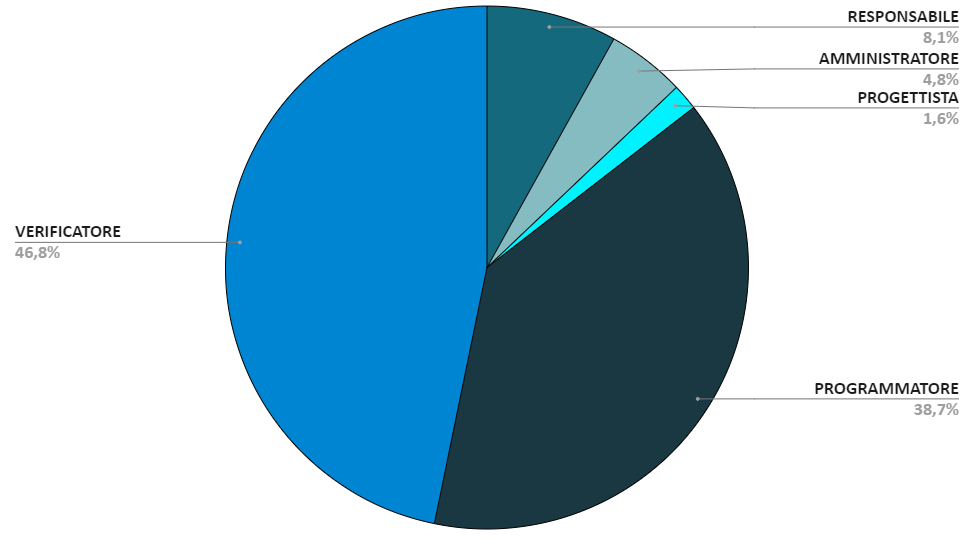
\includegraphics[width=0.8\textwidth]{prev11ruoli.png}
    \caption{Distribuzione dei ruoli undicesimo sprint}
    \label{fig:preventivoorario11sprint}
\end{figure}


\newpage

\subsubsection{Preventivo economico}

{
\setlength{\tabcolsep}{10pt}
\renewcommand{\arraystretch}{1.5}
\rowcolors{2}{oddrow}{evenrow}
\begin{table}[h]
    \centering
    \begin{tabularx}{\textwidth}{| l | l | l | X |}
        \hline
        \rowcolor{headerrow} \textbf{\textcolor{white}{Ruolo}} & \textbf{\textcolor{white}{Costo orario}} & \textbf{\textcolor{white}{Ore impiegate}} & \textbf{\textcolor{white}{Costo €}} \\
        \hline
        Responsabile & 30 & 5 & 150\\
        \hline
        Amministratore & 20 & 3 & 60\\
        \hline
        Progettista& 25 & 1 & 25\\
        \hline
        Analista & 25 & 0 & 0\\
        \hline
        Programmatore & 15 & 26 & 390\\
        \hline
        Verificatore & 15 & 31 & 465\\
        \hline
        \cellcolor{headerrow} \textbf{\textcolor{white}{Totale}} &  &  & \textbf{1090}\\
        \hline
        \cellcolor{headerrow} \textbf{\textcolor{white}{Rimanente}} &  &  & \textbf{895}\\
        \hline
    \end{tabularx}
    \caption{Preventivo economico undicesimo sprint}
    \label{tab:preventivocosti11sprint}
\end{table}
}

\begin{figure}[h!]
    \centering
    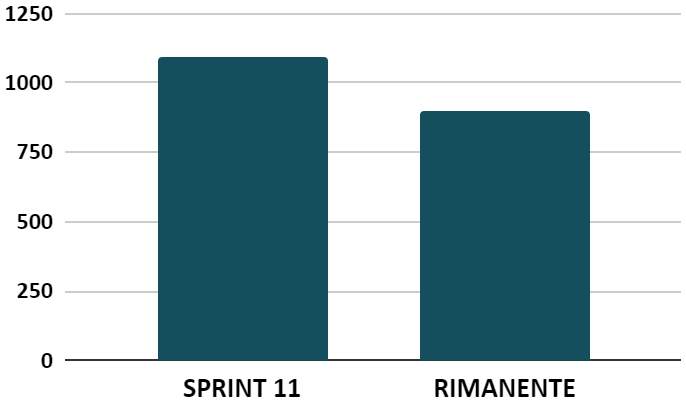
\includegraphics[width=\textwidth]{prev11costo.png}
    \caption{Costo preventivato undicesimo sprint e rimanente}
    \label{fig:preventivocosto11sprint}
\end{figure}

\newpage